\documentclass[12pt]{article}

\usepackage{hyperref}
\usepackage{graphicx}
\usepackage{longtable}
\usepackage[dvipsnames,table]{xcolor}

\graphicspath{{./img/}}

\definecolor{light-gray}{HTML}{E5E4E2}

\pagenumbering{arabic}

% VARIABLES
\def\UART_VERSION{v1.0.0}

\begin{document}
\begin{titlepage}
  \centering
  {\LARGE \textsc{Uart Implementation Reference}\par}
  {\vspace{1cm}}
  \UART_VERSION \\
  {\vspace{16cm}}
  Written by \\
  Kevin LASTRA
\end{titlepage}
\tableofcontents
\newpage

\section{Version}
\begin{tabular}{|p{1.5cm}|p{1.5cm}|p{2.5cm}|p{7cm}|}
  \hline
  \rowcolor{light-gray}\textbf{Version} & \textbf{Date} & \textbf{Author} & \textbf{Description} \\
  \hline
  v1.0.0 & 0 & Kevin Lastra & Initial release of the UART Implemenation Reference \\
  \hline
\end{tabular}
\newpage
\section{Introduction}
\subsection{Purpose of the manual}
The purpose of this manual is twofold. First, it serves as a 
comprehensive resource to document the Implementation of a 
Universal Asynchronous Receiver-Transmitter (UART). This process 
has been undertaken not only as a journey of self-learning but also 
as a way to share knowledge and contribute to the broader community
of developers, engineers, and enthusiasts.

\subsection{Audience}
This manual is primarly intended for design engineers who are 
involved in the development and implementation of communication
systems, particularly those working with embedded systems, 
microcontrollers, and hardware interfaces.

\newpage
\section{UART protocol overview}
The Universal Asynchronous Receiver-Transmitter (UART) is a 
fundamental hardware communication protocol used for asynchronous
serial communication. \\
This protocol is widely used in embedded systems, 
microcontrollers, and communication devices due to its simplicity and effectiveness
in handling relatively low-speed data transfer.
\subsection{UART fundamentals}
\subsubsection{Reception and transmission}
UART allows two devices to exchange data using only two wires, RX for receive data
and TX for transmit data.\\
\begin{figure}[h]
  \centering
  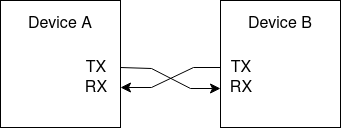
\includegraphics[width=0.6\textwidth]{UART_interface.png}
  \caption{Two UART's interfaces connected}
\end{figure}


\subsubsection{Asynchronous communication}
An asynchronous communication refers to a type of data transmission where the sender
and receiver do not rely on a shared clock signal for synchronization. Instead, each
device operates using its own internal clock and relies on specific timing 
conventions to ensure data is transmitted and received correctly. \\~\\
In asynchronous UART communication, the data is sent in discrete chunks 
(called data frames) over the communication channel, with the timing governed by 
agreed-upon parameters like baud rate and frame size.

\subsubsection{Baud rate}
The baud rate defines the speed at which data is transmitted over the communication
channel. It is usually expressed in bits per second (bps). \\
In the context of UART the baud rate specifies how many bits of data can be 
transmitted each second. Both transmitter and receiver must be set to the same baud
rate. \\~\\
The general formula for calculating the baud rate is:

\[Baud Rate = \frac{Clock Frequency}{Divisor}\]

\subsubsection{Data frame structure}
A UART data frame typically consists of: \\

\begin{table}[h]
  \centering
  \begin{tabular}{|p{3cm}|p{6cm}|p{3.5cm}|}
    \hline
    \rowcolor{light-gray}\textbf{Range name} & \textbf{Description} & \textbf{Implementation bit length} \\
    \hline
    Start bit & Signals the beginning of data transmission & 1 \\
    \hline
    Data bits & The actual data being sent & 5 - 9 \\
    \hline
    Parity & Used for error checking & 0 - 1 \\
    \hline
    Stop bit & Signals the end of the data transmission & 1 - 2 \\
    \hline
  \end{tabular}
\end{table}

\subsection{Advantages and limitations}
Advantages:
\begin{enumerate}
  \item Minimal pins required, essay to implement on a system.
  \item Low cost, because of its minimal hardware requirements the UART is a
        cost-effective solution.
  \item Widely supported.
  \item Simplicity in software implementation.
\end{enumerate}
limitations:
\begin{enumerate}
  \item Distance limitations, the maximum range depends on the baud rate, the quality
        of the wires and the environment (e.g. electromagnetic interferences).
  \item Relatively slow data transfer.
  \item Limited to two devices.
  \item Susceptibility to baud rate mismatch.
  \item Limited error detection, UART error detection is limited to parity checks and
        stop bits.
\end{enumerate}
\newpage
\section{Implementation}
\subsection{Design}
The UART implementation is composed of four primary modules: a Receiver, 
a Transmitter, a Clock Generator, and a control and status register with an 
AXI4 system interface.
\begin{figure}[h]
  \centering
  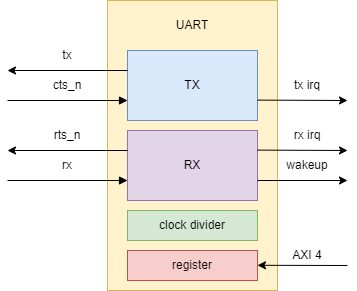
\includegraphics[scale=0.6]{UART_IMPL_DIAGRAM.png}
  \caption{Implementation diagram.}
\end{figure}

\subsubsection{Uart configuration}
\# TODO : configuration structure
\subsubsection{Data frame}
The received and transmitted data frame is built has follows : \\

\noindent \begin{tabular}{|p{3cm}|p{3cm}|p{3cm}|p{3cm}|}
  \hline
  \rowcolor{light-gray}\textbf{Start} & \textbf{Data} & \textbf{Parity} & \textbf{Stop} \\
  \hline
  1 & 8 & *1  & 1 \\
  \hline
\end{tabular} \\~\\
\noindent (*) The parity bit is an optional feature.
\subsubsection{Receiver (RX)}
This module is responsible for sampling and decoding incoming serial data. It 
detects the start bit, samples each data bit based on the configured baud rate, 
check the parity bit and verifies the stop bit. Once a complete and valid frame 
is received, the data byte is stored in an asynchronous FIFO for further 
processing by the system.

\# TODO : rx status

\subsubsection{Transmitter (TX)}
The transmitter handles the serialization of data from an asynchronous FIFO. 
It prepends a start bit, appends a parity bit and a stop bit, and transmits the 
bits sequentially according to the configured baud rate.

\# TODO : tx status

\subsubsection{Interrupts}
\# TODO : Explains when is latch and posedge event
\subsubsection{Wakeup line}
\# TODO : Explains when is latch and posedge event

\subsection{Control and status registers}

\noindent\begin{longtable}{|p{2.2cm}|p{1.4cm}|p{1.1cm}|p{1.1cm}|p{7cm}|}
    \hline
    \rowcolor{light-gray}\textbf{Register} & \textbf{Access type} & \textbf{Offset} & \textbf{Reset} & \textbf{Description} \\
    \hline
    divider & RW & 0x00 & 0x0 & Used to generate the UART clock by 
    dividing the system clock. \\
    \hline
    rx\_data & RO & 0x04 & 0x0 & Last received data. One-time read access. \\
    \hline
    rx\_status & RO & 0x08 & 0x0 & RX module status: \\
    & & & & \begin{tabular}{|c|c|}
              \hline
              \rowcolor{light-gray}Bit & Name \\
              \hline
              \rowcolor{white}
               0 & Fifo empty \\
               1 & Fifo full \\
               2 & Overrun error \\
               3 & Parity error \\
               4 & Framing error \\
              \hline
            \end{tabular} \\
    & & & & \\
    \hline
    rx\_irq\_mask & RW & 0x0C & 0x0 & Enables interrupts for specific bits in rx\_status \\
    \hline
    tx\_data & WO & 0x10 & 0x0 & Write data to TX asynchronous FIFO. If full overrun\_error 
    status will be set to 1. \\
    \hline
    tx\_status & RO & 0x14 & 0x0 & TX module status: \\
    & & & & \begin{tabular}{|c|c|}
              \hline
              \rowcolor{light-gray}Bit & Name \\
              \hline
              \rowcolor{white}
               0 & Fifo full \\
               1 & Fifo empty \\
               2 & Overflow error \\
              \hline
            \end{tabular} \\
    & & & & \\
    \hline
    tx\_irq\_mask & RO & 0x18 & 0x0 & Enables interrupts for specific bits in tx\_status \\
    \hline
    control & RW & 0x1C & 0x0 & Configure UART: \\
    & & & & \begin{tabular}{|c|l|}
              \hline
              \rowcolor{light-gray}\textbf{Bit} & \textbf{Name} \\
              \hline
              \rowcolor{white}
               0 & Flush tx FIFO \\
              \hline
               1 & Flush rx FIFO \\
              \hline
               2 & Enable/Disable flow control \\
              \hline
               3 & Enable/Disable parity bit  \\
              \hline
               4 & Master device. Used only \\ 
                 & on mode SIMPLEX or \\ 
                 & HALFDUPLEX. \\ 
                 & 1 - Use only TX line \\
                 & 0 - Use only RX line \\
              \hline
               [5:6] & Uart mode: \\ 
                     & 2'b00 : SIMPLEX \\
                     & 2'b01 : HALFDUPLEX \\
                     & 2'b20 : FULLDUPLEX \\
              \hline
            \end{tabular} \\
    & & & & \\
    \hline
    version & RO & 0x20 &  & Hold the current version implemented \\
    \hline
\end{longtable}

\subsubsection{Instantiation}
\# TODO :
\# Input and Outputs
\# Axi4 interface
\# Parameters

\subsubsection{Instantiation}
\# TODO : 
\# FMAX?

\end{document}